%%
%% This is file `sample-sigplan.tex',
%% generated with the docstrip utility.
%%
%% The original source files were:
%%
%% samples.dtx  (with options: `sigplan')
%% 
%% IMPORTANT NOTICE:
%% 
%% For the copyright see the source file.
%% 
%% Any modified versions of this file must be renamed
%% with new filenames distinct from sample-sigplan.tex.
%% 
%% For distribution of the original source see the terms
%% for copying and modification in the file samples.dtx.
%% 
%% This generated file may be distributed as long as the
%% original source files, as listed above, are part of the
%% same distribution. (The sources need not necessarily be
%% in the same archive or directory.)
%%
%% The first command in your LaTeX source must be the \documentclass command.
\documentclass[sigplan,screen]{acmart}
%% NOTE that a single column version is required for 
%% submission and peer review. This can be done by changing
%% the \doucmentclass[...]{acmart} in this template to 
%% \documentclass[manuscript,screen,review]{acmart}
%% 

%% TODO: there's still "Conference’17, July 2017, Washington, DC, USA" on every page after that :(
% https://tex.stackexchange.com/questions/346292/how-to-remove-conference-information-from-the-acm-2017-sigconf-template
\settopmatter{printacmref=false} % Removes citation information below abstract
\renewcommand\footnotetextcopyrightpermission[1]{} % removes footnote with conference information in first column
%\pagestyle{plain} % removes running headers

%% To ensure 100% compatibility, please check the white list of
%% approved LaTeX packages to be used with the Master Article Template at
%% https://www.acm.org/publications/taps/whitelist-of-latex-packages 
%% before creating your document. The white list page provides 
%% information on how to submit additional LaTeX packages for 
%% review and adoption.
%% Fonts used in the template cannot be substituted; margin 
%% adjustments are not allowed.
%%
%% \BibTeX command to typeset BibTeX logo in the docs
\AtBeginDocument{%
  \providecommand\BibTeX{{%
    \normalfont B\kern-0.5em{\scshape i\kern-0.25em b}\kern-0.8em\TeX}}}

%% Rights management information.  This information is sent to you
%% when you complete the rights form.  These commands have SAMPLE
%% values in them; it is your responsibility as an author to replace
%% the commands and values with those provided to you when you
%% complete the rights form.
%\setcopyright{acmcopyright}
%\copyrightyear{2018}
%\acmYear{2018}
%\acmDOI{10.1145/1122445.1122456}

%%TODO was mache ich hiermit?
%% These commands are for a PROCEEDINGS abstract or paper.
%\acmConference[Woodstock '18]{Woodstock '18: ACM Symposium on %Neural
%  Gaze Detection}{June 03--05, 2018}{Woodstock, NY}
%\acmBooktitle{Woodstock '18: ACM Symposium on Neural Gaze Detection,
%  June 03--05, 2018, Woodstock, NY}
%\acmPrice{15.00}
%\acmISBN{978-1-4503-XXXX-X/18/06}


%%
%% Submission ID.
%% Use this when submitting an article to a sponsored event. You'll
%% receive a unique submission ID from the organizers
%% of the event, and this ID should be used as the parameter to this command.
%%\acmSubmissionID{123-A56-BU3}

%%
%% The majority of ACM publications use numbered citations and
%% references.  The command \citestyle{authoryear} switches to the
%% "author year" style.
%%
%% If you are preparing content for an event
%% sponsored by ACM SIGGRAPH, you must use the "author year" style of
%% citations and references.
%% Uncommenting
%% the next command will enable that style.
\citestyle{acmauthoryear}

%%
%% end of the preamble, start of the body of the document source.
\begin{document}

%%
%% The "title" command has an optional parameter,
%% allowing the author to define a "short title" to be used in page headers.
\title{Gigapixel Imaging}
\subtitle{An Overview of the Technology and Related Technical Challenges}

%%
%% The "author" command and its associated commands are used to define
%% the authors and their affiliations.
%% Of note is the shared affiliation of the first two authors, and the
%% "authornote" and "authornotemark" commands
%% used to denote shared contribution to the research.
%\author{Ben Trovato}
%\authornote{Both authors contributed equally to this research.}
%\email{trovato@corporation.com}
%\orcid{1234-5678-9012}
%\author{G.K.M. Tobin}
%\authornotemark[1]
%\email{webmaster@marysville-ohio.com}
%\affiliation{%
%  \institution{Institute for Clarity in Documentation}
%  \streetaddress{P.O. Box 1212}
%  \city{Dublin}
%  \state{Ohio}
%  \country{USA}
%  \postcode{43017-6221}
%}

\author{Maria Shishkina}
\affiliation{%
  \institution{Cologne University of Applied Sciences}
  \streetaddress{Betzdorfer Str. 2}
  \city{Cologne}
  \country{Germany}
  \postcode{50679}}
\email{mashishkina@web.de}


%%
%% By default, the full list of authors will be used in the page
%% headers. Often, this list is too long, and will overlap
%% other information printed in the page headers. This command allows
%% the author to define a more concise list
%% of authors' names for this purpose.
%\renewcommand{\shortauthors}{Shishkina}

%%
%% The abstract is a short summary of the work to be presented in the
%% article.
\begin{abstract}
 Recent trends in the semiconductor technologies outline the possibility to acquire images with the resolution surpassing the physical limits of human perception. Resulting images lie in the gigapixel range; compared with the modern consumer electronics, the resolution of such sensors is higher by three orders of magnitude. 

Here, we explore a recent gigapixel imaging solution, the specialized sensor model with a  spectral sensitivity response and the spatial resolution nearing that of a photographic film. The pixels incorporated on an array converge to the theoretical minimum size limit -- to the point where their respective full well capacitance is limited to a photon each -- thus providing a non-linear binary response with the intensity distribution that adheres to the fundamental physical principles. To accommodate for the diffraction limits of optics, the sensor values are subjected to oversampling; temporal oversampling is possible as well to achieve better estimation of factual intensity values.

We present the image formation model of the quanta imaging sensor which should help simulate image capture in a sub-diffraction resolving light field. Later, we report on the most commonly advised method used for the image reconstruction and the parameters needed for accurate estimation with present noise sources. Due to the compact design of the photoelements, quanta imaging sensor provides high readout speeds with high resolution and inherits most of the advantages of the current state-of-the-art CMOS.



\end{abstract}

%% TODO
%% The code below is generated by the tool at http://dl.acm.org/ccs.cfm.
\begin{CCSXML}
<ccs2012>
   <concept>
       <concept_id>10010583.10010786.10010813.10010815</concept_id>
       <concept_desc>Hardware~Single electron devices</concept_desc>
       <concept_significance>300</concept_significance>
       </concept>
   <concept>
       <concept_id>10010583.10010786.10010810</concept_id>
       <concept_desc>Hardware~Emerging optical and photonic technologies</concept_desc>
       <concept_significance>500</concept_significance>
       </concept>
   <concept>
       <concept_id>10010583.10010786.10010787.10010788</concept_id>
       <concept_desc>Hardware~Emerging architectures</concept_desc>
       <concept_significance>300</concept_significance>
       </concept>
   <concept>
       <concept_id>10010583.10010588.10003247.10003250</concept_id>
       <concept_desc>Hardware~Noise reduction</concept_desc>
       <concept_significance>100</concept_significance>
       </concept>
   <concept>
       <concept_id>10010583.10010588.10003247.10003248</concept_id>
       <concept_desc>Hardware~Digital signal processing</concept_desc>
       <concept_significance>300</concept_significance>
       </concept>
   <concept>
       <concept_id>10010583.10010588.10010595</concept_id>
       <concept_desc>Hardware~Sensor applications and deployments</concept_desc>
       <concept_significance>100</concept_significance>
       </concept>
   <concept>
       <concept_id>10010583.10010588.10010591</concept_id>
       <concept_desc>Hardware~Displays and imagers</concept_desc>
       <concept_significance>500</concept_significance>
       </concept>
 </ccs2012>
\end{CCSXML}

\ccsdesc[300]{Hardware~Single electron devices}
\ccsdesc[500]{Hardware~Emerging optical and photonic technologies}
\ccsdesc[300]{Hardware~Emerging architectures}
\ccsdesc[100]{Hardware~Noise reduction}
\ccsdesc[300]{Hardware~Digital signal processing}
\ccsdesc[100]{Hardware~Sensor applications and deployments}
\ccsdesc[500]{Hardware~Displays and imagers}
\ccsdesc[300]{Mathematics of computing~Stochastic processes}

%%
%% Keywords. The author(s) should pick words that accurately describe
%% the work being presented. Separate the keywords with commas.
\keywords{gigapixel imaging, photon-counting, jot devices, binary image sensor model, SPAD, quanta imaging sensor}

%% A "teaser" image appears between the author and affiliation
%% information and the body of the document, and typically spans the
%% page.
\begin{teaserfigure}
  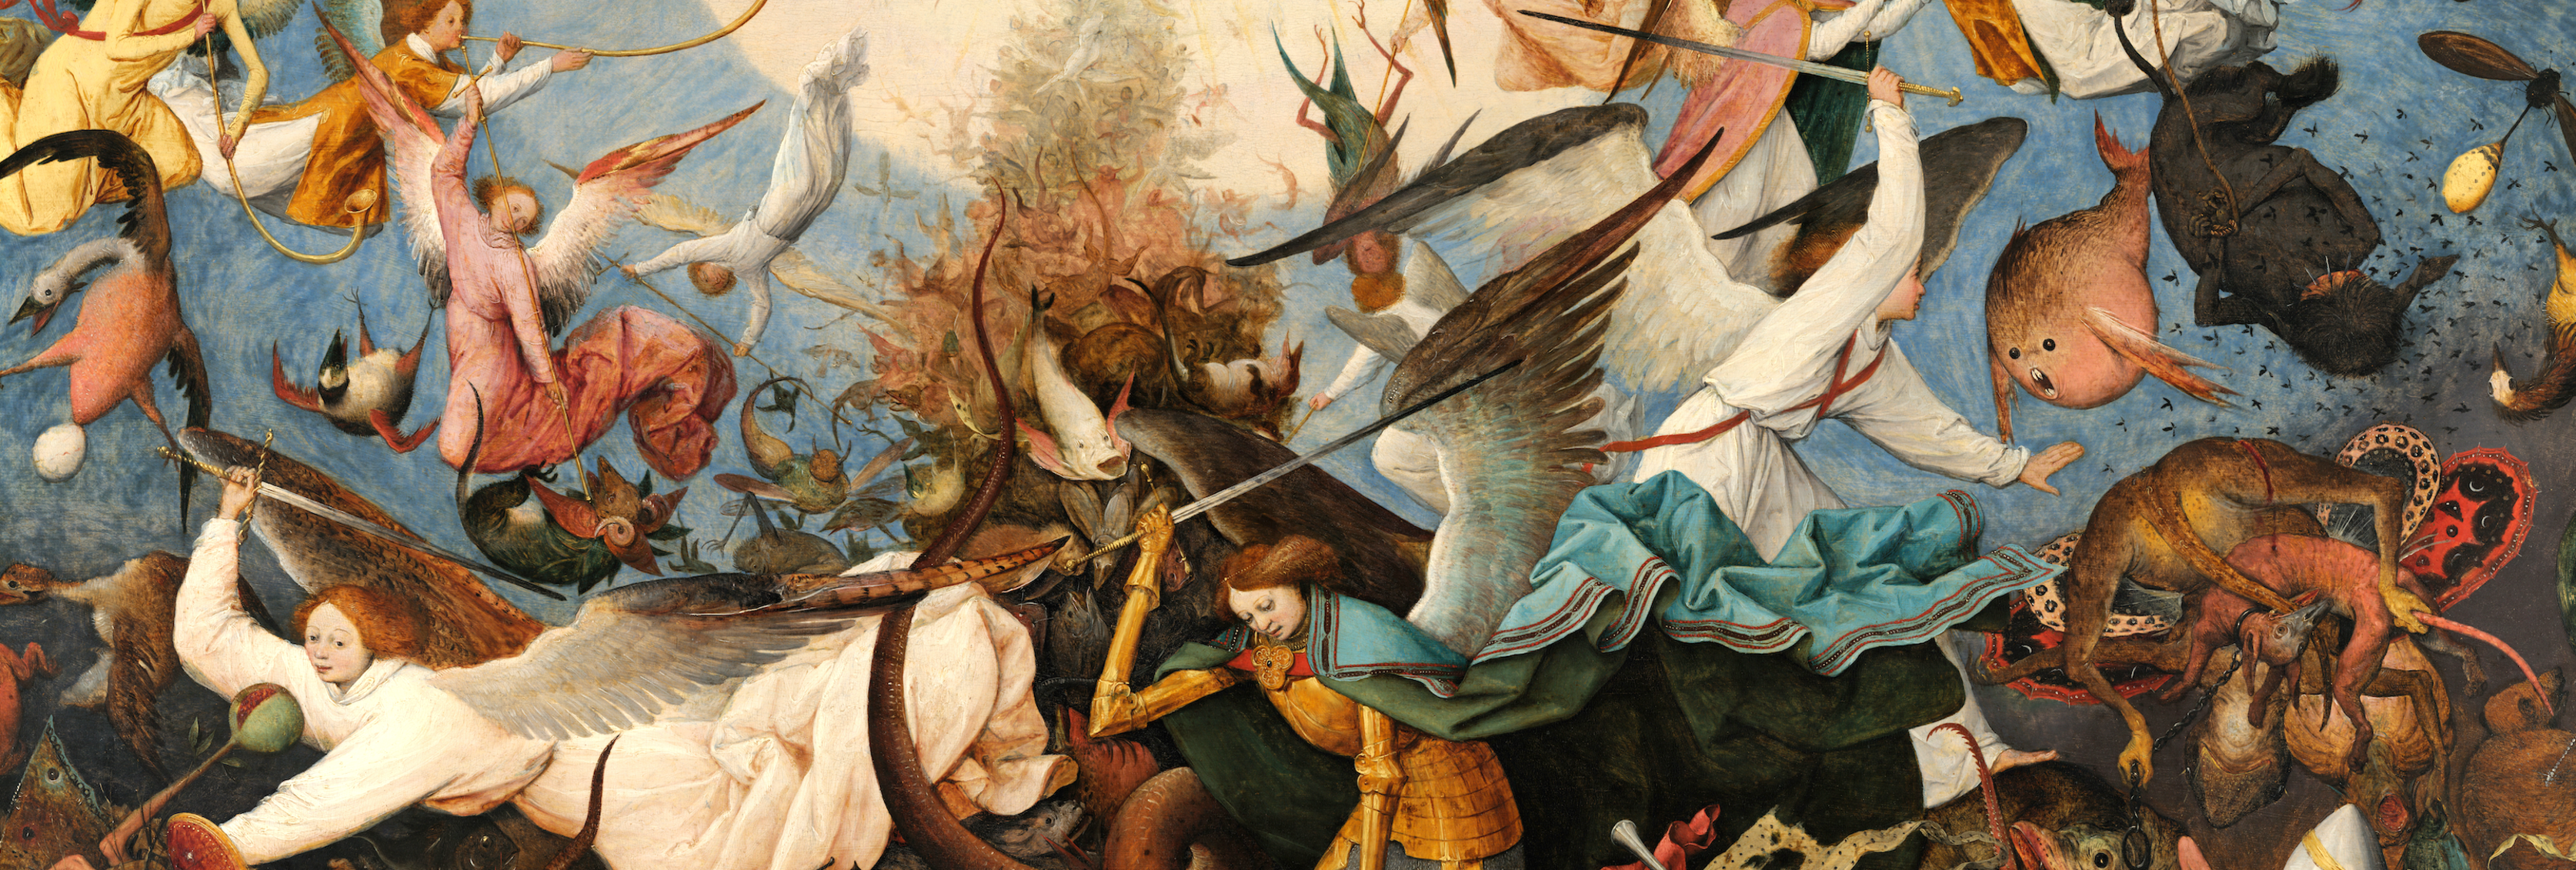
\includegraphics[width=\textwidth]{bruegel.pdf}
  \caption{Detail of the gigapixel image of Pieter Bruegel the Elder's \textit{The Fall of the Rebel Angels}, 1562, captured for Google Arts \& Culture. The full-resolution version of the image is sampled at 72 dpi with 30.000x21.654 px total. [Public domain], via Wikimedia Commons.
  (\url{https://commons.wikimedia.org/wiki/File:Pieter_Bruegel_the_Elder_-_The_Fall_of_the_Rebel_Angels_-_Google_Art_Project.jpg})}
  \Description{The gigapixel image of ``The Fall of the Rebel Angels'', the artwork by Pieter Bruegel the Elder. Oil on panel, 1562.}
  \label{fig:teaser}
\end{teaserfigure}
%%
%% This command processes the author and affiliation and title
%% information and builds the first part of the formatted document.

\maketitle

\section{Introduction}
%\section{Introduction}

\subsection{Motivation}
\label{chapter:motivation}

With every consecutive year, the information processing technologies advance in functionality and performance, leading to improvements in information capture, transmission, storage, and subsequent manipulations. 

In modern imaging devices, one of the most significant performance metrics is the spatial resolution of the system, expressed as the amount of resolvable information per unit of space. High resolution is crucial for distinguishing structures located within a small proximity to each other. Resolution improves with the shrinkage of the imaging elements, e.g. pixels in a sensor, and allows for more precise representations while potentially retaining the same system size in general. 

Such developments are generally desired: while not necessarily as significant for the most conventional consumer imaging devices, improved accuracy and reconstruction of the data is pivotal for a number of domains. These include remote sensing for astronomical imaging, microscopy research in biological sciences, prognostics, and medical examinations, and many more. Super-resolution is equally important in industrial applications, where the amount of data available for intepretation can be used in computer vision tasks such as object recognition or traffic surveillance.%, general prognostics, and medical examinations.
\cite{SResolution, Anwar2020ADJ}  

\subsection{State of the Art}
The current implementations tend to make use of the established digital sensor technology standard, the CMOS active pixel imaging sensor with intra-pixel charge transfer. Often described as a "camera-on-a-chip" technology, the conventional CMOS image sensor (CIS for short) has found use in both consumer and industrial applications due to its low-power consumption, high level of integration and small manufacturing sizes~\cite{8454568}. 

The highest resolution pixel-wise in current imaging devices is nearing 150 MP~\cite{lawton_artaius_2021}, where it's partially associated with larger sensor formats, sacrificing the compact size in the process for insignificantly larger amount of picture elements. High prices render such cameras unattainable for an average consumer. Besides the actual acquisition process, existing images have to be reconstructed in higher resolutions as well.

\subsubsection{Software-Based Implementations}

Many existing image processing approaches can be employed to enhance spatial resolution in existing \textit{low resolution} (LR) images. Based entirely in the software domain, such solutions require nothing but computational power and are utilized the most, to the point of being synonymous with the term ``gigapixel imaging'' itself.

The image recreation process is data-driven: the input can be a single image, or consist of a dataset of similar images with insubstantial differences from one another. Similarly, the methods employed can be based on the computer vision algorithms in the traditional sense or involve deep learning network architectures, which require an additional source of data in order to be outperforming the prior~\cite{Anwar2020ADJ}.

\paragraph{Image Stitching}

Image stitching techniques explicitly require abundant, spatially and temporally coherent image datasets with overlapping regions. The most common application of such techniques consists in the production of high-resolution panoramic images, which can then be   utilized for entertainment or preservation purposes~\cite{7136690}.

By now, the production of the panoramic gigapixel images is steadily made available to the consumers. A fine example is the GigaPan technology~\cite{GigaPanWWW}, which stems from the collaboration between Carnegie Mellon University, NASA Robotics Group, and Google; since then, it has been spun off into a commercial service offering both hardware accommodations and the software, thus defining a clear, streamlined workflow. The solutions encompass a designated robotic mount facilitating continuous image capture through panning along its axis, a corresponding image stacking software, and even a web-based interface for sharing the composite image afterwards. 

The camera mount is meant for use with any amateur DSLR camera, meaning that the exact resolution of the resulting panorama is dependent on the dimensions of the optical components and the sensor model. The demonstration of the process can be found online \cite{GigaPanVimeo}.

\paragraph{Image Synthesis via Deep Learning}

Deep learning-

based methods are best employed for a reconstruction of a single low-resolution image. 

The super-resolution version of a single image is by definition an under-determined problem with a multitude of possible solutions. Classical computer vision algorithms don't fare well in such tasks, as the recovery of such images may lead to the propagation of wrong information. For an accurate reproduction of the scene, one may need reliable prior information which relates to the human perception in a meaningful way. 

The objects depicted in the image can be upsampled based on their predicted taxonomy and feature sets, which is one of the main applications of the convolutional neural networks. Depending on the data involved in the training, the interpolated data could be refined in many ways; for instance, distinguished objects could have their corresponding surfaces refined based on their class, filling in the structures with already available high-resolution textures of the corresponding materials.

A number of network designs, varying widely in their complexity, depth, training data, and features, has been considered for the gigapixel imaging. An extensive overview on the available architectures can be found in \cite{Anwar2020ADJ} and \cite{10.1007/978-3-030-36808-1_37}.
 
 
\paragraph{Applicability}

One should note that neither image stitching nor image synthesis techniques are exclusive to the gigapixel imaging in their methodology; working with a sequence of images in particular is a challenge which quickly turns into an image registration problem, requiring integrated solutions regarding tonemapping, uneven illumination, projective distortions of the depicted objects etc. For this reason alone, the strictly software-based solutions pose no special challenge to the gigapixel imaging and are therefore declared out of scope of this paper.

\subsubsection{Hardware-Based Implementations} 

The computational complexity of the problem can be reduced by addressing it on a lower level of abstraction. Here, the focus lies on acquiring the super-resolution directly by means of the appropriate hardware architecture design. With this, the need for elaborate LR datasets lapses as well. 

Several solutions focusing on the predominantly hardware-based domain exist. %underlying analog circuit components
 
\paragraph{Scanning}

A popular imaging solution involves a flatbed scanner capable of relatively high scanning resolution (commonly provided in dots per inch, or DPI): with most consumer scanning devices supporting 300 dpi and above, this off-chip solution is both low-cost and widely available. 
 \begin{figure}[h]
  \centering
  \includegraphics[width=0.7\linewidth]{imgs/gigascan.png}
  \caption{The proof-of-concept gigapixel microscopy setup, as demonstrated in \cite{zheng20140}. The scanner at hand can resolve 2400dpi, which corresponds to the pixel size of ca. 10$\mu$m.}
  \label{fig:gigamicro}
  \Description{Proposal for a gigapixel imaging setup for usage in microscopy. Depicted are generic flatbed scanner, a lens, and a sample to be captured. The sample is illuminated and positioned next to the optical system such that a magnified image appears, projected onto the scanning area.}
\end{figure}

In gigapixel solutions tailored specifically to microscopy research, the scanners register magnified projections of the input samples \cite{Zheng:12};
% previously magnified via a  closed-circuit-television lens
other papers attempt to enhance the scanning process by modifying the scanner device directly \cite{ConfocalScan}, or using alternative scanning methods (e.g. tilt scanning in \cite{tileScan}).

 %\begin{figure}[h]
%  \centering
%  \includegraphics[width=\linewidth]{imgs/scantech.png}
%  \caption{Tilt scanning techniques presented in \cite{tileScan}.}
%  \Description{Scanning can be performed diagonally, where the new direction doesn't fit the singular pixels exactly, and each detector fits somewhere in the middle. Through such incoherences, one can oversample the light field similar to the phase shift method.}
%\end{figure}

%Projection-based scan methods may contain redundancies depending on the source. For instance, light intereference should be taken into account; with analog media, one risks introducing further factors into the equation, as the optical density in a print image will also depend on the properties of the photographic medium (paper, ink, etc.), the device used for printing, and present physical foreign particles, such as dust. In this case, the quantity does not necessarily substitute the quality, and the higher spatial resolution merely leads to the redundancies in data, thus not influencing the information content itself in any way.

\paragraph{Composite of Sensor Arrays}
An attempt to attain high resolution in the digital domain using existing technologies is a popular method in large scale applications. 

Widely used in airborne and astronomical systems are precision-mosaicked sensor arrays. In this case, conventional MP-sized imaging sensors are brought together into an array and treated as a whole. Since the optical components of the system are mostly unchanged, this is a fixed-focus system. %; similarly, the same step can be applied to preceding optical components of the system. 

Such cascading architectures are rather unwieldly, expensive, and is therefore mostly found in research facilities, where the rigidity of the architecture is unimportant. This stacked sensor technology can be seen in airborne and astronomical systems such as ARGUS, LSST and Pan-STARR~\cite{multiscale}.

Alternatively, the system can employ multicameras, allowing for a multi-scaled approach. One of such gigapixel camera architectures is AWARE, developed by The Duke Information Spaces Project. AWARE employs arrays of microcameras, using a monocentric lens objective as the primary optical component. The first generation, AWARE-2, consisted of 98 microcameras on a monochromatic CMOS sensor, producing a 1.0 gigapixel image spanning a 120$\deg$ × 40$\deg$ field of view~\cite{GongGPU}. Since then, a variety of models have been developed, enabling color acquisition and ranging in optical resolution, size, and amount of microcameras. There are operational advantages to AWARE as well, since each camera can be independently controlled in acquisition settings~\cite{multiscale}. Summarized, such multilens cameras are more compact and serve well in terrestrial applications. \cite{aware2}

 \begin{figure}[h]
  \centering
  \includegraphics[width=0.5\linewidth]{imgs/aware.jpg}
  \caption{AWARE-2 camera design, via: \cite{physics_world_2018}}
  \Description{AWARE-2, one of the multilens camera designs presented in the paper}
\end{figure}

\paragraph{Photon-Counting}
The latest advancements in the manufacturing of integrated circuits (ICs) have put us in the post-Moore's law era. 

From 1970s on \cite{Cerofolini2007}, the complexity of the circuitry would grow at a much higher rate than once theorized, while the physical dimensions of the semiconductors would scale down. By 2020, the possible pixel pitch in CMOS sensors can be as low as 3$n$m~\cite{hao2021recent}, meaning that the sensor dimensions used in current photographic devices can now hold significantly larger pixel amounts, providing us with higher spatial resolution in an image. However, at the present time the pixel dimensions are approaching physical limits: by reducing the pixel area, the full-well [photoelectron charge] capacity of a singular pixel, too, is lowered. This has grave implications for the image quality, as the small difference between the signal and the noise decreases the dynamic range. 

The solution to overcoming the trend of pixel shrinkage while maintaining the higher resolution has been proposed by Eric R. Fossum in 2005.%, an inventor of CMOS. 

Sufficiently small pixels should only be able to store charge of one photoelectron alone.  Each of those pixels can then assume values of either 0, meaning no photons have reached the light-sensitive sensor plane, or 1, signifying that at least one has struck the surface after all, resulting in registered exposure. The sensor response lies in a binary range. The actual evaluation of the sensor data, i.e. the image formation, happens post-capture via analysis of the Poisson distribution of the photons over multiple observations in time, and can be managed dynamically. 

Photon-counting, or, quantum imaging sensors can ultimately represent a paradigm shift in photography. Since its introduction, the binary sensor has been applied and conceptualized in many ways.% Such devices will be the main focus of this report. 


\section{Theoretical Background}

\subsection{Light Propagation}

The electromagnetic radiance is expressed through the flow of minute particles, or quanta, named \textit{photons} in the context of light. The energy of a single photon, \begin{equation}W = h \cdot v \: \textup{[J]}\end{equation}
is a product of the frequency $v \:\textup{[Hz]}$, and the Planck constant $h = 6.62607015 \cdot 10^{-34} 
\:\textup{J\:s}$, valid for every harmonically oscillating system.


%\subsubsection{Quantum Fluctuations of Light}

Photons arriving at each pixel can be approximated by a Poisson  distribution function and arrive at random times. The rate of the photon arrivals, i.e. the distribution of the photons, is however still dictated by the local light intensity, as seen in Figure  \ref{fig:photon}. 

%$$\mathbb{P}\left\{B_{m}=1 ; s_{m}\right\}=\mathbb{P}\left\{Y_{m} \geq q ; s_{m}\right\}=\sum_{k=q}^{\infty} \frac{s_{m}^{k} e^{-s_{m}}}{k !}$$

\begin{figure}[h]
  \centering
  \includegraphics[width=\linewidth]{imgs/optics/photon.png}
  \caption{Random photon arrival time, modeled with two optical power sources. Even for a constant source, the arrival is probabilistic. Adapted from \cite{Saleh1991}.}
  \label{fig:photon}
  \Description{Two diagrams depicting behavior of registered photons in time depending on the variations in optical power.}
\end{figure}

\subsection{Photoelectric Effect in Sensors}

%The charge within each pixel on a sensor is collected through the estimation of the photons impinging on the respective pixel surface, inversely proportional to the capacitance ....
%A photon with energy hν breaks a silicon bond and frees both an electron (e-) and a hole (e+).
Imaging electronic devices consist of arrays of pixels, consisting of photodiodes accumulating charge through incoming light and integrated circuits which read out the charge and process it further.

For the accumulation of charge, the properties of the semiconductor materials are exploited. 
The unique electrical conductivity of semiconductors can be altered significantly through external sources of energy, e.g. thermally or by light illumination, and increases proportionally. 

The incident photons impinge on the surface of the image sensor and are absorbed through the corresponding structures in the semiconductor material, creating electron-hole pairs as the electron is excited from the valence to the conduction-band. The photoexcited carriers remain within the sample; this is called \textit{internal photoeffect}. \cite{Saleh1991} %645 & 576 %to the higher energy level.

Electrical and optical properties of the semiconductors can be altered further through \textit{doping}, an adding of local impurities for changed concentration of the carriers. In semiconductors, selective doping creates an electrostatic potential well. Subjected to the externally applied electric field, the freed photoelectrons drift through the material towards the potential well, where they are stored and integrated for the duration of exposure. This photoelectron charge is later transferred to the sense capacitance, thus producing measurable electric current through changes in the charge on the charge sense node (\textit{floating diffusion} FD) and converting the signal to voltage, which is read out by the a source follower transistor. \cite{9059308} %their charge is converted to voltage via transfer to a sense capacitance, change in the charge on this sense node causes change in voltage, thus converting the signal from charge domain to voltage domain

The outputs of the source-followers are amplified and fed to the signal processing circuits on a greater scale, allowing the separate pixels to be adressed column-wise. After the integration, the pixels are reset.

\begin{figure}[h]
  \centering
  \includegraphics[width=0.9\linewidth]{imgs/sensors/3tppd.png}
  \caption{3T PPD structure, via \cite{Holst2011}. Typically, the dark current is heightened through the direct n+ contact; here, this is prevented through p+-pinning structure on the pixel surface.}
  \label{fig:3tppd}
  \Description{The classical pinned photodiode structure with three nodes.}
\end{figure}

Many implementations for the photodiodes exist. In the simplest pixel circuit, three transistors (3T: source-follower, reset, and row select transistors) are needed for the integration process. Modern CIS technologies make use of 4T pinned photodiode structure, in which an additional transfer gate is positioned between photodiode and the sense node. This ensures reduction of dark current and complete charge transfer; the ``pinning'' of the photodiode allows for reduced sense node capacitance. 
Furthermore, with this design structure, the pixels can be reset simultaneously, allowing for same integration periods globally.

\begin{figure}[h]
  \centering
  \includegraphics[width=0.9\linewidth]{imgs/sensors/4tppd.png}
  \caption{4T PPD structure, via \cite{Holst2011}. The transfer gate provides isolation of the regions.}
  \label{fig:4tccd}
  \Description{The pinned photodiode structure with four transistors. There are slight differences regarding the placement of the wells and the junctions, as the n+ is now spatially separated from the n-.}
\end{figure}

Only a fraction of the incident photon flux is absorbed and brought to a higher energy level. The ratio of the photoelectrons to the incident photons is given by \textit{quantum efficiency} (QE), which often ranges from 50\% to 80\% \cite{9059308}.
The relationship between the changes in output voltage caused by the photoelectric effect to the number of photoelectrons is given by conversion gain (CG); in modern CIS devices, this typically amounts to 100$\mu$V/$e^{-}$~\cite{7006672}. 


\subsection{Noise Modeling in Digital Sensors}


The noise, that is, unwanted deviations in the signal, can be comprised of the multiple sources which are subsequently added throughout the digital image acquisition chain. Deviations in the brightness are introduced right in the detection phase due to the discrete nature of electrons; such noise source is dubbed photon shot noise. Further fluctuations are caused during the readout of the electron charge and its subsequent amplification; for digital systems, the mapping of the voltage to discretized bit values results in the additional quantization noise. \cite{Holst2011}

\begin{figure}[h]
  \centering
  \includegraphics[width=\linewidth]{imgs/sensors/sens-signal-transfer.png}
  \caption{Signal transfer diagram in an imager, via \cite{Holst2011}. Both analog and digital outputs are considered.}
  \label{fig:sigtrans}
  \Description{Signal transfer diagram in a digital sensor. There are multiple subsystems leading to the accurate normalized representation of the signal: at first, the incident photons are detected and evaluated in their charges; this is later amplified and digitized.}
\end{figure}

\begin{figure}[h]
  \centering
  \includegraphics[width=\linewidth]{imgs/sensors/sens-noise-transfer.png}
  \caption{Noise transfer in a digital sensor, via \cite{Holst2011}. Each subsystem introduces additional noise sources which affect the subsequent signal.}
  \label{fig:noisetrans}
  \Description{For every subsystem listed in the signal transfer diagram, there is a corresponding noise source which alters the input: the photon-induced noises, reset noises, noises caused through amplifiers (off-chip and on-chip), and finally, the quanification noise.}
\end{figure}

Figures \ref{fig:sigtrans} and \ref{fig:noisetrans} show the signal transfer and the noise occuring during each step of the process, respectively. Each noise source has a different characteristics and can be attributed to either nonuniformities and physical flows of the sensor, or the natural nonstationary processes. The level of detail in the noise transfer diagram is somewhat dependent on the application, and some of the sources caused by the circuitry can be minimized through the design of the architecture, as will be shown in the further chapters. 

\subsection{General Requirements in Gigapixel Applications}

Several general requirements must be met in gigapixel imaging devices. Since the higher information efficiency is desired in both scientific and consumer-grade applications (see Section \ref{chapter:motivation}), a high-resolution camera must not differ drastically from current implementations in its imaging capability.

For components which are primarily influenced by optoelectrics, \cite{GigaOptik} name following requirements:

\begin{itemize}
    \item a \textit{field of view} (FOV) of at least ca. 40$^\circ$, which is equivalent to the angle of view for humans at infinity focus ($\mathrm{FOV} = 2 \times \arctan\left(\frac{\text{sensor size}}{2{f}'}\right)$, ${f}' = 50m$m),
    \item an f-stop of ca. f/4-f/11 for operation under most common lighting conditions,
    \item and a lens design with low complexity to facilitate both portability and low manufacturing costs.
\end{itemize}

\subsection{Diffraction-Limited Systems}% (→ comparison with classical optics)

\label{chapter:diff}

In a typical imaging system, before arriving at the sensor, the incident light is collected and focused through an optical system first. Lenses, most common optical components, have a resolving power of their own, which has to match the resolution of the sensor and is fundamentally limited by the nature of light. 

Upon encountering an opening (\textit{aperture}), the incident light diffracts into a series of concentric waves propagated concentrically around the corners. Assuming a perfectly circular aperture, wavefronts belonging to one point in object space will produce a diffraction pattern with a bright spot in the middle, surrounded by concentrical rings of reduced intensities. The diameter of such pattern, \textit{Airy disk}, is given through:

\begin{displaymath}
    D_{Airy} \approx 2.44 \frac{\lambda {f}'}{D} = 2.44 \lambda  k
\end{displaymath}

with $\lambda$ being the wavelength of the incoming light, ${f}'$ the focal length, and $D$ the diameter of the entrance pupil, respectively; in lenses, which can be treated as a circular aperture of respective diameter, the \textit{focal ratio} serves as the \textit{nominal aperture} $k$, or \textit{f-stop}. 

\begin{figure}[h]
  \centering
  \includegraphics[width=\linewidth]{imgs/optics/airy.png}
  \caption{Airy disk pattern caused through lens diffraction of a point source, via \cite{Cagnet1962}, and and the corresponding distribution of intensities, \cite{Demtroeder2018}.}
  \label{fig:airy}
  \Description{The bundle of light passing through a lens, acting as an aperture. Through diffraction, the points in the object plane are depicted as a concentric wave-like pattern of diminishing intensities.}
\end{figure}

For two distant neighboring points, the half-angle ${\delta}'_{min}$ subtended by the numerical aperture (represented by the lens) is too small. Thus, the two objects will not be perceived as separate entities; as their intensity functions coincide at their respective minimums, the disks will start to overlap. 

\begin{figure}[h]
  \centering
  \includegraphics[width=\linewidth]{imgs/optics/airy-limit.png}
  \caption{The imaging subsystem is not capable of resolving two adjacent object points, leading to the interferences in the signal. Via \cite{Cagnet1962} and \cite{Demtroeder2018}.}
  \label{fig:airylimit}
  \Description{Two point sources are depicted in an imaging system and raytraced in a manner similar to the previous figure. The limits placed by diffraction cause the concentric patterns to overlap, rendering the two point sources spatially indistinguishable from each other.}
\end{figure}
%also, numerical aperture = n sin delta, with n = 1 bc air
The angular resolution of an optical system in an object plane is concomitant with a spatial resolution in an image representation, due to to the small-angle aproximations \cite{Pedrotti2007}. Defined via \textit{Rayleigh criterion}, the least resolvable distance between two points should correlate with the distance between the two peaks of the intensity distribution function (as seen in Figure \ref{fig:airylimit}):

\begin{displaymath}
  {\delta}'_{min} =  1.22 \lambda \frac{{f}'}{D} = 1.22 \lambda k \simeq {\rho}'_{\infty } 
\end{displaymath}

The latter is defined as the resolution limit ${\rho}'_{\infty}$ and can be approximated for the near field application, where the distance ${a}'$ between the aperture and the sensor plane is larger than the focal length ${f}'$:

\begin{displaymath}
{\rho}'_{near}  =  1.22 \lambda \frac{{f}'}{D} \frac{{a}'}{{f}'}= 1.22 \lambda k (1 - {\beta}' )
\end{displaymath}

The resolution limit presented earlier sets a limit for the peak lens performance, which varies with the fundamental physical quantities, like wavelength range and focal ratio.  
Further limitations are imposed through the geometric aberrations, caused by the physical imperfections in the optics itself.

The number of distinct resolvable points for a lens is defined by the \textit{space-bandwidth product} (SBP) \cite{Cossairt:11} and ties the lens performance to the sensor size.

\cite{GigaOptik} state two common approaches for enhancing the SBP. Those consist of either scaling the system up, or introducing further optical surfaces to the imaging system for better lens performance. The scaling can occur in either one of the subsystems, meaning an integration of a sensor with larger dimensions or scaling the lens.%, which are said to have SBP quadratic... aus scaling laws 
The second measure should lessen influence of geometric aberrations, leading to a diffraction-limited performance; however, the increased complexity of the optical system implies higher manufacturing costs and errors due to misalignment. Detailed description of scaling laws for the lenses is provided in \cite{Cossairt:11}, who account for both diffraction-induced limits and geometric aberrations.

As the CIS pixel sizes are routinely surpassing the 1.5$\mu$m extent, the optical system in a gigapixel application is doomed to have a lower resolving power than the sensor itself even if the lens performance is solely diffraction-limited; hence, the resolution in image space will be limited through optics. Resulting image representations contain spatial redundancies due to the light field being oversampled. 

While many proof-of-concept solutions exist that aim to enhance the resolution on a solely optical level (i.e., multiscale design and monocentric lenses), computational post-processing in gigapixel devices might turn out to be compulsory.


\section{Photon-Counting Detectors}
%\section{Binary sensor imaging}
\subsection{Photon-Counting in Film Photography}

The principal notions of the single-bit imaging sensors can be traced back to analog photography and demonstrate behaviors reminiscent to ones of the silver halide emulsion, a common component in the photographic film. 

Akin to its digital counterpart, the photographic film is subjected to the photoelectric effect; in film, this is represented by the photographic emulsion coated on the transparent sheet of plastic. Such emulsion consists of microscopic crystals, or grains, of silver halides embedded in protective colloid like gelatin \cite{Carroll1980}, with the commonly considered compounds being silver bromide \textit{AgBr}, silver chloride \textit{AgCl}, silver iodide \textit{AgI}, or some mixture thereof \cite{Schroeder1981}.
%ionenbindung löst photographischen primärprozess: elektron durch quantenenergie abgespalten; wirkung des primproz ist srtreng proportional zu der quantenzahl!
\begin{figure}[h]
  \centering
  \includegraphics[width=0.5\linewidth]{imgs/film/silver.jpg}
  \caption{Electron microscopic structure of undeveloped silver bromide crystals, via \cite{AgfaABC}.}
  \label{fig:silverbromide}
  \Description{Small blackish crystals of silver on gray background}
\end{figure}

The process starts upon exposure of the film to the light. Film grains absorb the incoming radiation in form of the incident photons and dissociate into a group of free silver ions. 

Once exposed to development agent, the silver ions in the film are reduced to metallic silver, rendering the exposed regions of the film sheet opaque black. The unaltered halides are later dissolved out in a chemical bath, so that the corresponding spots are transparent. Each crystal can either be struck by a photon or not, and so the film exhibits a binary response. 

%chance of absorprtion of a photon by a grain; grain must absorb r quanta in order to be developable. when r = 1, equation is reduced to 1-e ^ (-q); the shape of the characteristic curve depends on photon distribution
The exposed grains are spread randomly, fluctuate in size and differ in absorption rate -- there is no uniformity regarding the required absorbed quanta as the particles arrive randomly. However, with the irradiance of the image areas varying, so does the stochastic photon distribution and therefore the concentration of silver particles per film area. 

Fine granular structures are not perceivable by the human eye and are registered as continuous tone of gray \cite{Feng_Yang_2012} instead, matching the overall area density to the original light intensity information; the mean number of absorbed quanta per grain is given by the Poisson equation. % (optical density)

%For conventional sensors some of this non-linear response can be encoded in the postprocessing of the linear-response image. Nevertheless, the non-linear response of film has been hard to match even in HDR solid-state image sensors without introducing artifacts due to motion, threshold voltage fixed- pattern variation, and other circuit design issues

\begin{figure}[h]
  \centering
  \includegraphics[width=\linewidth]{imgs/film/filmcurve.jpg}
  \caption{Exemplary characteristic curve of the film emulsion, via \cite{Saleh1991}.}
  \label{fig:filmcurve}
  \Description{S-shaped curve relates the optical density to the logarithmic exposure. There are two latitudes on both ends of the curve.}
\end{figure}
The photographic properties of the film emulsion are typically described through the ratio of the luminance transmitted in the medium to the luminance of the observed scene. The optical density is modelled as a function of logarithmic exposure and was first derived in \cite{HurterDriffield}. As seen in Figure \ref{fig:filmcurve}, this relationship has a non-linear behavior. 

The D - log H curve (also referred to as \textit{ characteristic curve}) can be split into three intervals based on the curvature of the response. For sufficiently small or large values of logH, the function is asymptotic and results in under- or overexposure (the toe and shoulder portions of the curve, respectively~\cite{Hunt2005}); in the middle interval, the slope is constant, and the relationship between the luminance and the photographic density is linear. %Under sparse exposures and overexposures, this means better tolerance for highlights
In general, the S-shape of the curve is determined by the underlying randomness of photon arrivals. (This is different in conventional CIS sensors.)

In film, the grains may fluctuate in size, ranging from 0.048 to 1.71 $\mu$m depending on the application; on average, one grain of the developed emulsion corresponds to ca. 3-4 electrons~\cite{Carroll1980, FossumSiMulQIS}. Feature sizes of QIS are similar in their capacitance; the jots in the single-carrier implementation of QIS are meant to store around 3 carriers as well. Thus, both digital sensors QIS and analog film deliver quantized, spatially discrete values obtained off similar area sizes. So, the behavior in binary imaging sensors is, too, dominated by the photon distribution. Resulting characteristic curve is shaped comparably, demonstrating slightly larger overexposure latitude~\cite{FossumSiMulQIS}.

\begin{figure}[h]
  \centering
  \includegraphics[width=\linewidth]{imgs/film/qiscurve.png}
  \caption{Characteristic curve of the quanta imaging sensor, via \cite{fossum2016quanta}.}
  \label{fig:qiscurve}
  \Description{Shown is the response of the QIS with the S-shaped curve relating the bit density to the exposure.}
\end{figure}


\subsection{SPAD Matrices}

The binary response of the sensor defines the need for a subsequent signal amplification process to generate a sufficiently large voltage signal from a single photon. In one of the currently available gigapixel imaging technologies, this is achieved via the integration of the \textit{single-photon avalanche diode} (SPAD) structures, which implement gain mechanisms internally (\cite{Saleh1991}); this internal amplification process is referred to as electron \textit{avalanche multiplication}~\cite{Ma:17}. Since each detected photon is converted into a cascade of moving carrier pairs, even weak light can produce a clearly detectable current. %The depletion-layer electric field in a photodiode is increased by applying a sufficiently reverse bias across the junction so that the electrons and holes generated may acquire sufficient energy to liberate more electrons and holes within this layer by a process of impact ionization. \cite{Saleh1991} 

\begin{figure}[h]
  \centering
  \includegraphics[width=0.8\linewidth]{imgs/avalanche.png}
  \caption{SPAD operation process, demonstrating changes in voltage during the avalanche effect and subsequent quenching. Via \cite{Charbon2018}}
  \label{fig:avalanche}
  \Description{A diagram shows the shift in current during the SPAD-based acquisition process, which happens rapidly for a single photon. Later, the current must drop via quenching.}
\end{figure}

In avalanche photodiodes, the junction electric field is large enough such that the available carriers are accelerated, causing \textit{impact ionization}, i.e., producing further photoelectrons through collision. Ergo, high electrical voltage over 20V is required~\cite{Gnanasambandam_2019}; some prototypes, like the one described in \cite{rng16}, define even higher supply voltages of ca. 22–27V for biasing above breakdown. SPAD is operated in Geiger mode \cite{7117471}. For SPAD arrays, higher breakdown voltage is desirable in general, as it allows for higher photon detection efficiency and improved timing resolution~\cite{7117471}.

The first proposal for a fully integrated CMOS SPAD array has been reported in \cite{Rochas2003}. \cite{DuttonSPAD} allude to other SPAD detectors which have been developed since, noting the variety in both general form (single-point detectors, line sensors, large array photomultipliers, and image sensors) and pixel designs; subsequently, it is stated that no single SPAD-based pixel architecture has been deemed dominant to date. 

The fast detection times in SPADs are associated with the rapidity of the impact ionization process. However, each photon detection event must be followed by finite recovery time, in which the diode is restored to the operative level voltage-wise, freeing excess charge carriers. This process is called \textit{quenching}. During this time, device does not respond to further incident photons. To enable quenching, additional in-pixel circuitry is needed.
Due top the larger amount of transistors needed per single photodetector, the fill-factor of SPAD-based pixels is limited (<40\%), and so is the quantum efficiency (<30\%)~\cite{Ma:17}.

Generally, the SPAD devices aren't entirely compatible with the CMOS technologies due to high operating voltage requirements; the necessity for a large electric field and additional readout circuitry results in the larger dimensions of the structure, lower spatial resolution and higher power dissipation~\cite{Ma:17}. Furthermore, the generation of electrons is based on thermal reactions, rendering the detectors significantly more susceptible to dark current.

However, significant progress has been achieved in recent years~\cite{SPADperformance, rng16}. Performance of SPAD-based architecture using the developments in 3D stacking technologies is described in detail in \cite{Charbon2018}.



\subsection{The Pixels as Jots}

The avalanche-mode operation in SPAD-based photodetectors limits the pixel pitch and the manufacturing yield and delivers highly undesirable amounts of dark current, which can be somewhat reduced through cooling. In fact, the abstinence from the avalanche photodiode technology is stated to be one of the design criteria in photon-counting applications.
Quanta imaging sensor (or QIS for short), a different implementation of the binary image sensor, attempts to overcome such limitations\cite{Ma:17, Ma03rmsJot}.
The principal advantages of CMOS arrays (low-voltage operation, low power consumption, ease of integration of on-chip operation control, the possibility of random access to the image data, etc., \cite{Holst2011}) must be retained. %S.105

In QIS, the photodetectors are intentionally made small as to be capable of storing charges of several electrons. 
Placed together in a structure, these become \textit{jot devices}, with "jot" denoting the ``smallest thing'', a word of Greek origin \cite{FossumSiMulQIS}.

In some of the available research (\cite{s16111961}), jots are referred to as subpixels, or, partitions of conventional CMOS memory bit-cells; other sources (\cite{fossum2016quanta}) may use the term ``\textit{SDL pixels}'', referring to the pitch values within sub-diffraction limit (200-500$n$m).

The jot photoelements have a \textit{small full-well capacity} (FWC, or storage capacity density, often provided in photoelectrons per cm$^2$), which ranges from one to around 100 or 200 carriers -- compared with the state-of-the-art conventional imaging sensors where the full well is first reached at ca. 4000$e^{-}$~\cite{Gnanasambandam_2020}, the values are low. Subsequent circuitry discriminates the output to one of the binary states \cite{FossumSiMulQIS}, based on the pre-defined, semi-arbitrarily set threshold $q$. 

Instead of converting the number of photons impinging on the sensor surface to voltage, either 1 or 0 are transferred and quantized. Precision of quantization is not of essence. The thresholds are set lower due to the relatively small FWC, and the binary response is triggered quickly. Thus, unlike conventional CIS pixels (described as "buckets" accumulating and integrating [larger] charges of multiple photoelectrons), jots require lesser integration times and can be readout at rates as high as 1000 frames, or fields, per second. 

\cite{MaJotDevices} envision QIS to have structures consisting of 0.1...10.0 Gjots; due to the fast readout speeds, dimensions of this order must lead to data rates of 0.1...10 Tb/s.

Research regarding the quanta imaging sensor technology is currently in progress. A prototype of camera featuring QIS has already been produced, albeit with a lesser spatial resolution and pixel pitch than sought-after. Representing a crucial paradigm shift, this imaging technology has full potential to stand in as the third generation of digital sensors, replacing CMOS. The benefits, advantages, and the detailed methodology behind QIS will be discussed in the remainder of this paper.

\section{Quanta Imaging Sensor}
\subsubsection{Jot Data Structure}
%Frames readout off the sensor are accounted for during the image formation, allowing for estimation of the local light intensities as a function of time.

\begin{figure}[h]
  \centering
  \includegraphics[width=\linewidth]{imgs/sensors/binarysensor.png}
  \caption{Binary sensor model, via \cite{Feng_Yang_2012}.}
  \Description{Photon-counting process in an oversampled binary sensor.}
\end{figure}

The output of the simple QIS design is binary in nature. Combined output of the QIS jots is a series of bit planes, observed over time. Since both spatial and temporal sampling take place, the output can be conceptualized as a cube, as shown in Figure \ref{fig:jotcube}.

\begin{figure}[h]
  \centering
  \includegraphics[width=0.7\linewidth]{imgs/qis/jotdatacube.png}
  \caption{Jot data cube, via \cite{fossum2016quanta}}
  \label{fig:jotcube}
  \Description{The output of a quanta image sensor, divided into binary values corresponsing to the spatial $x$-$y$-coordinates and the temporal dimension $t$.}
\end{figure}

Unlike CIS arrays which produce images of fixed sizes, quanta imaging sensor allows the output pixel image size to be programmable and dynamically adjustable~\cite{FossumSiMulQIS}; the image reconstruction mostly occurs post-acquisition, and the bit plane can be divided into smaller jot cubicles of arbitrary sizes which should then form a single pixel in the conventional sense from temporal and spatial data.

It is understood that the forming of the image pixels does not require uniformly sized jot cubicles; for separate pixels, these can have different dimensions in $x$, $y$, and $t$. It follows that selected cubicles of the adjacent pixels may overlap, aiding formation of multiple CIS pixels at once~\cite{fossum2016quanta}.

\subsection{Distinctions}

The similarity of the QIS response to the sensitivity of the photographic film emulsion has been established in the previous sections; in both cases, the shape of the characteristic curve is determined by the photon arrival statictics. 

In film, around 3-4 carriers were needed to elicit the chemical reaction. Since the binary value is obtained through comparisons against a certain threshold, the choice of threshold can influence the final response. Figure \ref{fig:qiskt} shows the response curves plotted for the number of carriers $k_{T}$ needed for the single-bit pixel output of ``1'' ($k_{T}=1,2,3,4,20$). It is evident that the linearity of the QIS response curve changes with the larger thresholds; similarly, the overexposure latitude is shifted towards larger exposures. Hence, the single-bit jot devices can be applicable under multiple varying lighting conditions, enabling low-light and high dynamic range imaging applications, where the acqusition using multiple threshold values would provide different values for linearity.

\begin{figure}[h]
  \centering
  \includegraphics[width=\linewidth]{imgs/qis/multicarrier.png}
  \caption{Single-bit QIS response curves in dependence of the amount of carriers, via \cite{FossumSiMulQIS}}
  \label{fig:qiskt}
  \Description{Response curves of QIS depending on the threshold. For larger values, the slopes are narrower, and the overexposure latitudes are reached upon stronger illumination, albeit more quickly.}
\end{figure}

For this reason, it is convenient to distinguish between the single-bit jot devices with full-well capacitances in the classical sense, of only one electron (\textit{single-carrier}), and multiple electrons (\textit{multi-carrier}) which can be dynamically adjusted in their responses based on the threshold.

\subsection{Hardware Design}

To facilitate the transition to the QIS as the future dominant sensor technology in the future, strong compatibility with a CIS fabrication line must persist.

CMOS sensor serves as a suitable basis for quanta imaging due to its low voltage specifications, high quantum efficiency, high spatial resolution, and more. \cite{Ma:17}. 
However, due to the source-follower output voltage, the read noise is too high to enable photon detection. Current state-of-the-art CIS demonstrate read noise in the ranges of 1...2$e^{-}$ r.m.s. ~\cite{7273747}. Due to the binary nature of the signal, such amount of noise has grave consequences for the single-bit QIS, resulting in high possibilities of false misquantization. At low light levels, desired read noise in single-bit QIS should amount to 0.3$e^{-}$ r.m.s. at best, delivering error-free estimation with 0.15$e^{-}$ r.m.s. under especially sparse exposures (0.01<H<1). For such low bit error rates, conversion gain of at least ca. 1$m$V/$e^{-}$ is needed, which is five times higher than the values demonstrated in the state-of-the-art CIS devices~\cite{MaJotDevices}.
For this reason, current CIS technologies must be modified in order to enable photon-counting.

%Instead of using avalanche gain to detect single photoelectrons, the gain comes from using a very small sense node capacitance yielding CG in the range of 500uV/e-. Using intrapixel charge transfer, a single electron transferred to that capacitance can produce a signal that is well above the noise floor (e.g. 0.2e- rms noise floor) and thus give a low error rate for detection of single photoelectrons. The detection process is slower than for SPADs, but sub-microsecond timing is achievable. Further, avoiding the high electric fields of SPADs enables smaller pixels or jots, improved manufacturability, and thus lower cost per pixel and smaller optics. Power dissipation is also considerably smaller. In late 2017, Dartmouth reported a 1Mpixel QIS device implemented in a nearly standard CMOS BSI stacked process with 1.1um pixel pitch, operating at 1000fps and dissipating about 20mW total power. The 1Mpixel QIS was demonstrated more than two years earlier than the 1Mpixel SPAD array and with much less development time and with much smaller pixels. About 73 CMOS QIS pixels can fit into the area of one SPAD pixel. This is the strength of working in nearly standard CMOS image sensor processes. The applications of QIS are currently being explored but include low-light imaging for security, defense and science.
%\cite{9059308}

%Single jot is described having storage well of 1...200$e^{-}$. 
During the charge-to-voltage conversion, the signal transfer is corrupted by noise  due to the voltage fluctuations and the parasitic capacitances in the circuitry, which reduce the transfer efficiency. %may end up corrupted by noise 
Higher conversion gain ensures that the estimations are accurate, and the transferred electrons are capable of producing signal above the noise floor. This could be achieved by increasing the voltage, however, higher operating voltage would render the sensor incompatible with most baseline CMOS processes.\cite{Ma:17} Otherwise, one can attempt to minimize the read noise, which is caused by the capacitance of the floating diffusion. In available works, FD is minimized via specialized jot structures, where the doping profiles of the pixels are modified via implantations.
Jot candidates based on their doping properties are covered in detail \cite{Masoodian16, Ma:17}. On average, the doping profiles of the jots have lead to the reduction of the noise to ca. 0.21$e^{-}$ r.m.s. with the conversion gain nearing 350$\mu$V/$e^{-}$ with 15\% variation~\cite{Ma:17}.

Most of the publications referenced in this work explore prototypes for jot devices which were fabricated in conformance with the 45/65nm 3D stacked CMOS process with backside-illumination (BSI), which guarantees high fill factor and quantum efficiency~\cite{Ma03rmsJot}.

Figure \ref{fig:qischip} demonstrates the architecture of existing 1Mjot clusters with vertical integration. The jot device is vertically separated from the readout circuitry, which reduces the total area and allows faster readout. Presented array can be implemented with analog and digital readout circuitry; Such clusters can be arranged in parallel, thus forming a chip of significantly larger dimensions without any significant delays in speed. In this particular jot device, analog clusters were integrated together with the digital clusters.

%Above all, in order to achieve the theorized performance, the jots must achieve higher conversion gain, and the appropriate architecture for the binary analog-to-digital-converter must be found to ensure that the resulting read noise is in the deep sub-electron range.

%Quanta imaging sensor inherits CIS advantages in terms of pixel size, spatial resolution, dark current, quantum efficiency (QE), readout speed, and power dissipation. Beyond CIS and existing photon-counting technologies, the QIS aims to realize accurate photon counting without avalanche gain or cooling, while maintaining low dark current and manufacturing cost.\cite{Ma:17}

\begin{figure}[h]
  \centering
  \includegraphics[width=\linewidth]{imgs/qis/mjot-wafer.png}
  \caption{Simplified architecture of the 1 Mjot stacking QIS chip (left) and one digital cluster (right), via \cite{Ma:17}}
  \label{fig:qischip}
  \Description{The wafer containing the photodetectors is positioned vertically above the circuitry. The jots are united in clusters, each cluster has a designated circuitry unit for readout.}
\end{figure}

\begin{figure}[h]
  \centering
  \includegraphics[width=0.5\linewidth]{imgs/qis/20Mjot.png}
  \caption{QIS test chip featuring 20 1Mjot arrays (left), via \cite{s19245459}.}
  \label{fig:20mjots}
  \Description{Yellow sensor chip realizing 20 Mjot clusters. The clusters are placed in a grid on the sensor plane.}
\end{figure}

Within a single-bit QIS, ADC acts as a simple comparator with an exposure-appropriate threshold $q$. Since the response is binary, the bit depth of only 1 is required for quantization.

\subsection{Multi-Bit QIS}

The field readout rate of the sensor can be traded off for the increased bit depth of the ADC, thus allowing to count more photoelectrons per each readout cycle. Such implementation of the sensor, the multi-bit QIS, can be seen as the middle ground between the conventional CIS and the single-bit photon-counting sensor~\cite{ADCmultibit}. The carrier numbers, which were previously reduced to single-bit values, can now be mapped to their respective quantities in a certain range. Upon saturation, the maximum number of the converter is reported instead~\cite{FossumSiMulQIS}.

Through lowered framerates and increased electron resolution, the output data transfer rate can be lowered. The increase in complexity of the ADC is negligible in comparison with the lowered complexity of the calculations; since the represented number of carriers is defined to be in the range of 1...200$e^{-}$, the resolution of the ADC does not need to be overly high, presenting significant improvements with the bit depth of $n = 6$. Reduction of the framerate for a multi-bit QIS occurs by the factor $2^n -1$; assuming the framerate of 1000 fps for single-bit QIS, the framerate of a multi-bit QIS will amount to $\frac{1000 \textup{fps}}{2^{n}-1}$, ensuring reduction by the factor of 63 in case with the 6b ADC.

Another advantage provided by the bit depth selection is the ability to adjust linearity and compression between the input photon flux and the output signal.

The prototype in Figure \ref{fig:20mjots} features 20 1Mjot arrays, allowing easy and flexible scaling in overall resolution due to the cluster-parallel architecture mentioned earlier. However, with each integrated arrays, the power dissipation is multiplied accordingly. The choice of ADC architecture for multi-bit QIS in terms of power consumption has been evaluated in \cite{ADCmultibit}, where the successive approximation register ADCs were deemed too be the least power-consuming option in relation to the occupied area. 


\subsubsection{Color Imaging}

Spectral information in digital sensors is typically obtained using \textit{color filter arrays} (CFAs), semi-transparent masks integrated on top of the sensor. These form a 2D periodical pattern with the three primary colors. Thus, each pixel is limited to irradiance related to the wavelength range of the respective color.

Later, the intensity values in each 2D kernel are reconstructed and interpolated, or \textit{demosaicked}, to form a single pixel with three colour channels.

The most widely used CFA configuration is Bayer RGB pattern, though many other arrangements exist~\cite{Krig2014}. Figure \ref{fig:cfabayer} shows the Bayer pattern and its exemplary position on a sensor plane.

\begin{figure}[h]
  \centering
  \includegraphics[width=0.8\linewidth]{imgs/cfa/cfabayer.png}
  \caption{Bayer RGB pattern and the common integrated CFA arrangement (right, via \cite{Krig2014}).}
  \label{fig:cfabayer}
  \Description{Pattern of Red, Green, Green, Blue is placed on top of the electronics.}
\end{figure}

Following problems pertain through inclusion of color information via CFA:

\begin{itemize}

\item \textbf{Aliasing}. Through demosaicking, combined spatial resolution is lowered, and under sampling rates below the Nyquist frequency, \textit{Moiré artifacts} appear.

\item \textbf{Reduced sensor sensitivity}. Part of light is blocked out and never reaches the sensor plane, and the net signal is more susceptible to noise.

\item \textbf{Crosstalk}. The optical or electrical charge in the pixels may leak towards the adjacent pixels. In CFAs, where charges depend on wavelengths and change rapidly, this results in a desaturation of the color measurements.
\end{itemize}

While these problems appear in monochromatic sensors as well, here, the errors persisting translate to false color values, which is more disturbing for the human perception \cite{Hunt2005}.

Not all effects are equally pronounced, however, attempts to alleviate one factor may result in higher impact of the others. For one, QIS sensors are unaffected by aliasing due to their small feature sizes, while conventional CMOS sensors may require designated algorithmic suppression. At the same time, smaller pixel pitches lead to severe crosstalk; even more so when the adjacent colors are different~\cite{elgendy2019color}, which is the case with the Bayer pattern. In binary sensors, the leakage means false positives, resulting in a substantially lower SNR.

\cite{Anzagira2015ColorFA} attempt to mitigate the crosstalk through the extensions of Bayer pattern. 

\begin{figure}[h]
  \centering
  \includegraphics[width=0.7\linewidth]{imgs/cfa/cfaqis.png}
  \caption{CFA Proposals made in \cite{Anzagira2015ColorFA}.}
  \label{fig:cfaqis}
  \Description{Squared patterns for color imaging, which now include more secondary colors in the arrays or the larger bounds of the primary colors in the pattern masks.}
\end{figure}

Figure \ref{fig:cfaqis} depicts two of the proposals. On the left, the initial mosaic is expanded through secondary colors cyan, magenta, and yellow. These are positioned between the respective primary colours so that the spectral overlap is smaller. For increased light sensitivity, some of the green pixels may also be replaced with white. The second proposal expands the active color regions of the filter, leveraging the high spatial resolution of the QIS. The overlaps now occur in the regions where the pixels are halved, which can be accounted for during computations.

%Assume cross-talk to be equal for all wavelengths and only pertain in vertical and horizontal directions

\cite{elgendy2019color} focus on more than merely crosstalk mitigation, proposing design criteria for sub-diffraction limit CFAs.
Paired with a demosaicing algorithm, this should maximize spatial resolution between the channels while improving the sensitivity in general. Similarly, the demosaicking process should minimize the noise power after the light passes the filter. 

Presented in Figure \ref{fig:cfaelgendy}, the filter has a diagonal structure. The auxiliary demosaicking algorithm works on frequency selection and was found to be universally applicable, performing well in both CIS and QIS imagers.

\begin{figure}[h]
  \centering
  \includegraphics[width=0.7\linewidth]{imgs/cfa/cfaelgendy.png}
  \caption{CFA pattern proposed in \cite{elgendy2019color}. The patterns are positioned diagonally, with gradations, as to reduce the cross-talk between the pixels.}
  \label{fig:cfaelgendy}
  \Description{Primary colors in the pattern are positioned diagonally}
\end{figure}

In both cases, the filter kernel is larger, and the spatial resolution of the sensor is traded off for better performance in presence of crosstalk. 


 \begin{figure}[h]
  \centering
  \includegraphics[width=0.5\linewidth]{imgs/qis/gigajot.png}
  \caption{Quanta imaging sensor, as seen in a Gigajot camera. Via: \cite{Gnanasambandam_2019}}
  \Description{Small industrial camera with equally small lens above it}
\end{figure}

The strictly algorithmic processing of the color image in QIS has been described and applied in \cite{Gnanasambandam_2019}, who present the QIS Pathfinder camera module developed at Gigajot Technology with a Bayer pattern color filter array implemented on-chip. 


\subsection{Compared Performance}

Table \ref{tab:comp} shows some of the most significant operating parameters for the two photon-counting sensor implementations. We have collected these specifications based on the state-of-the-art implementations of the devices reported in the references section, taking the values from the most recently published sources in case of ambiguities.

It is evident that while SPAD-based arrays have higher dark current through thermally-induced avalanche gain, their read noise is still rather low, and the framerate is higher than the one in QIS by several orders of magnitude. The reasons for this behavior, i.e. the amount of circuitry required to implement quenching, were mentioned in detail in previous sections. The read noise in QIS is nearing the ideal, relatively error-free value of 0.15$e^{-}$ r.m.s., while the dark current is completely negligible.

\begin{table}
  \caption{Comparison of QIS and SPADs}
  \label{tab:comp}
  \begin{tabular}{l|cc}
    \toprule
    Parameters & QIS & SPAD\\
    \midrule
    Pixel pitch & 1.1$\mu$m & 5-10$\mu$m\\
    Read noise [RT] & 0.21$e^{-}$ r.m.s. & <0.15$e^{-}$ r.m.s.\\
    Dark current [RT] & 0.16$e^{-}$ r.m.s. & >10$e^{-}$ r.m.s.\\
    Framerate & 1040 fps & 97 000 fps \\
    Quantum efficiency & 70-80\%  & 30-50\% \\
    Fill factor & >90\% & <70\% \\
    Full well capacity & 1-200$e^{-}$ & N/A \\
    Operating voltage & 2.5/3.3V & 15-25V\\
    \bottomrule
  \end{tabular}
\end{table}

The contrast in approaches is noticeable in almost every other specification. Compared to QIS, SPADs need high electrical voltage to accelerate the photoelectrons, while providing lesser quantum efficiency. Such differences provide a clear distinction between the applications of both photon-counting sensors: SPAD-based imaging is significantly more functional in applications that value acquisition rate above all and need better temporal resolution, e.g. Time-of-Flight imaging, while QIS is better suitable for applications that prioritize accuracy and low-light sensitivity. Low-light imaging applications of QIS may include astronomy, surveillance, medical examinations, and many others. With sufficiently large oversampling, the single-bit QIS can have substantially higher dynamic ranges, being able to acquire scenes containing both bright and dark regions~\cite{Feng_Yang_2012} and benefitting from the non-linear binary curve. According to \cite{9059308}, about 73 CMOS QIS pixels can fit into the area of one SPAD pixel, rendering the technology especially desirable in microbiology purposes.

\section{Image Formation in a QIS}
%\subsection{Image Formation}
\label{chapter:imform}

%The gigapixel implementation of QIS is still in the proposal phase. The current prototypes of the quanta imaging sensors incorporate around 10Mjots. However, the concept of the image reconstruction following the initial readout of the sensor data does not indicate any possible complications through scaling of the array dimensions; the principles employed during post-processing are governed by the same physical processes and presume the sources of error of the same magnitude.

The image formation process in a QIS imaging sensor consists of two fundamental processing blocks and can be seen in Figure \ref{fig:qismodel}. For reasons of simplicity, we present the model based on the single-bit sensor.

\begin{figure}[h]
  \centering
  \includegraphics[width=\linewidth]{imgs/qis/qis-model.png}
  \caption{QIS image formation model, via \cite{s16111961}.}
  \label{fig:qismodel}
  \Description{The image reconstruction model for QIS applications.}
\end{figure}

The first block comprises operations necessary to perform spatial oversampling of the diffraction-limited light field. In the second block, the upsampled light undergoes the binary sensing, where the exposure values are filled in using the one-bit quantized Poisson statistics.

It should be noted that the temporal oversampling is omitted in this particular figure, though it is foreseen by definition.

\subsection{Spatial Oversampling of the Light Field}

Assuming $N$ discrete spatial coordinates, i.e. the amount of observable pixels per unit space, the light intensities are a vector of coefficients in discrete space $\boldsymbol{c}=\left[c_{0}, \ldots, c_{N-1}\right]^{T}$. For convenience, we consider the variables to be acquired in a one-dimensional space, i.e., a vector $\boldsymbol{c}_{N \times 1}$. 

The signal is assumed to be normalized to prevent scaling ambiguity such that $c_n \in [0,1]$. In order to achieve the proper range scaling for the observations, the inputs are upscaled via multiplication with the factor $\alpha > 0$, representing the \textit{sensor gain}. Afterwards, the existing data is ready to be spatially upsampled with the specified degrees of freedom needed for the modelling. 

Depending on the total amount of jots $M$, every observation $c_n$ is multiplied by the \textit{spatial oversampling factor} $ K \stackrel{\Delta}{=} \frac{M}{N} $; every diffraction-limited pixel is subsequently spread out outwards. It is per definition that the $K \in \mathbb{Z}^{+} $.

The missing intensity values are filled in via lowpass filtering with a discrete, non-negative kernel $\boldsymbol{g}$; a common choice for an interpolation kernel is the box-car function, which is defined such that it's coefficients are
\begin{equation}g_k = \frac{1}{k} \;\textup{for} \;k = 0, 1, ... , K-1.\end{equation}

Although other lowpass filtering operators are available (\cite{Feng_Yang_2012} name cardinal B-splines and squared sinc function), boxcar function is assumed to be the most accurate emulation of the oversampled light field: due to the microlenticular lenses placed in front of the jots in most functioning prototypes, it can be safely assumed that the light is focused on each jot.\cite{qisthreshold}

Assuming the sampling is performed using the box\-car filtering function, one can describe the entirety of the oversampling process as a sequence of linear operations; the aforementioned operations can therefore be concatenated und rewritten in the form of $\boldsymbol{s} = \alpha \boldsymbol{G}_c $, corresponding to a matrix-vector multiplication with the filter response function $\boldsymbol{G}_c$ of the interpolation filter in the Fourier domain.

\begin{figure}[h]
  \centering
  \includegraphics[width=0.8\linewidth]{imgs/qis/jotdatasimulation.png}
  \caption{Oversampled light field simulation. Via: \cite{fossum2016quanta}}
  \label{fig:jotdata}
  \Description{The common image of Lenna has film-like qualities due to being oversampled using Poisson statistics.}
\end{figure}

\subsection{Binary Sensing}

The oversampled light field, already provided in discrete form, has to be approximated further by simulating the light fluctuation throughout the jot device and the subsequent thresholding. 

The fluctuations, i.e. the photon shot noise, adhere to the Poisson distribution. In measurements over an arbitrary period of time $t$, the probability of obtaining $y_{m}$ photoelectrons is based on exposure $s_{m}$ like
\begin{equation}\mathbb{P}\left\{Y_{m}=y_{m} ; s_{m}\right\}=\frac{s_{m}^{y_{m}} e^{-s_{m}}}{y_{m} !}\end{equation}

%\begin{equation}\mathbb{P}\left\{k\right\}=\frac{e^{-H}H^{k}}{k !}.\end{equation}
%$\mathbb{P}\left\{B_{m}=1 ; s_{m}\right\}=\mathbb{P}\left\{Y_{m} \geq q ; s_{m}\right\}=\sum_{k=q}^{\infty} \frac{s_{m}^{k} e^{-s_{m}}}{k !}$
The quantization process is a mapping of detected photoelectrons into the binary range, based on the non-negative threshold $q$: $B: \mathbb{Z}^{+} \cup\{0\} \longmapsto\{0,1\}$.

\begin{equation}\boldsymbol{B}(y) \stackrel{ \Delta }{=}\left\{\begin{array}{ll}1 & \text { for } y \geq q \\ 0 & \text { otherwise }\end{array}\right.\end{equation}

For a threshold of $q = 1$, the probabilities of no photon arrivals are therefore estimated as 
\begin{equation}\label{eq:poisson0}\quad \mathbb{P}\left\{B_{m}=0 ; s_{m}\right\}=e^{-s_{m}} \quad\end{equation}leaving us with $\mathbb{P}\left\{B_{m}=1 ; s_{m}\right\}=1-e^{-s_{m}}$ otherwise.

%\subsubsection{Non-Linearity and the Bit Density}
%\label{chapter:nlbd}
%\cite{FossumSiMulQIS} manages to relate the probabilities of detection to the sensitivity response of QIS, and does so on a larger scale, observing clusters of multiple jots.

%In a single-bit photon-counting sensor, the probability of no arrivals is given via Equation \ref{eq:poisson0}. For $M$ uniformly illuminated jots, the number of jots with such state is $M \times e^{-s_{m}}$, or $M \times e^{-H}$; remaining jots with the response of 1 are $M \times (1- e^{-H})$, accordingly.

\subsection{Error Rates}
In the presented model, only natural photon shot noise is considered~\cite{Feng_Yang_2012, s16111961}. Generally, the signal transfer chain is much closer to the equation

\begin{equation}\boldsymbol{x}_{\mathrm{QIS}}=\operatorname{ADC}\{\text { Poisson }(\alpha \cdot \boldsymbol{x}_{\text {true}}+\boldsymbol{\eta}_{\mathrm{dark}}))+\boldsymbol{\eta}_{\mathrm{read}}\}\end{equation}

and the photon noise is less dominant under sparse exposures. 

Generally, there is also read noise, introduced by the readout process through the readout circuit transistors (resulting in flicker noise, 1/f) and reset on capacitors. These are critical in low-light imaging conditions, where the number of photoelectrons is sparse. The readout noise is often referred to the equivalent number of input photoelectrons.\cite{7422662}. 

In a normalized uncorrupted signal \begin{equation}
U_{s i g} \triangleq \frac{V_{s i g}}{C G}
\end{equation}
the value is only dependant on the number of photoelectrons readout, i.e. the \textit{electron number}, and is Poisson distributed. There is equivalence between the interpretation of the electron number and the ratio of the voltage to conversion gain $CG$.

However, assuming additional read noise, normalized as
\begin{equation}
    u_{n} \triangleq \frac{v_{n}}{C G}
\end{equation}

the probability distribution function depends not just on obtaining a certain amount of photoelectrons, but the noise $u_{n}$ as well. Since the read noise is best approximated through Gaussian, the total probability is a convolution of the Poisson distribution for quanta exposure H (equivalent to $s_m$ in previous chapters) and a normal distribution with read noise $u_n$. 

\begin{equation}\mathbb{P}[U]=\sum_{k=0}^{\infty} \frac{\mathbb{P}[k]}{\sqrt{2 \pi u_{n}^{2}}} \exp \left[-\frac{(U-k)^{2}}{2 u_{n}^{2}}\right]
\end{equation}

When $U_{sig}$ is quantized with a 1b analog-to-digital-converter, it is subjected to a comparison with a threshold $U_{th}$, commonly 0.5~\cite{FossumSiMulQIS}. With fluctuations caused by read noise, the binary response is prone to errors. 
We are presented with two options: either there are no electrons, but the 0 is misquantized as 1 due to the added noise, or there is a positive response of 1 misquantized as 0. The sum of these false positives and false negatives in ratio to total number of jots is the \textit{Bit Error Rate} (BER).

\begin{figure}[h]
  \centering
  \includegraphics[width=0.8\linewidth]{imgs/ber.png}
  \caption{Bit Error Rate in single-bit sensors, via \cite{FossumSiMulQIS}.}
  \label{fig:berrate}
  \Description{Two parabolic functions with overlaps in the middle of the chart. The overlap characterizes the erroneous measurements}
\end{figure}

In Figure \ref{fig:berrate}, the misquantizations are shown for the single-bit case with a threshold exactly in the middle. There are only two possible states, and for each state, there's a possibility of an error. The false estimations are formed in the overlapping section.

The false negatives and false positives are obtained through the integration of the probability distribution function,
which leads us to expressing these as an error function:

\begin{equation}
    P_{f n}=\frac{1}{2} \operatorname{erfc}\left[\frac{1-U_{t h}}{\sqrt{2} U_{n}}\right]
\end{equation}
and
\begin{equation}
P_{f p}=\frac{1}{2} \operatorname{erfc}\left[\frac{1}{\sqrt{8} U_{n}}\right]
\end{equation}

When the threshold is put exactly in the middle, the false positives and false negatives are equally probable. The total bit error rate with the threshold of $U_{th}=0.5$ amounts to 

\begin{displaymath}
B E R=\frac{1}{2} \operatorname{erfc}\left[\frac{1}{\sqrt{8} U_{n}}\right]\end{displaymath}

and is only acceptably small with read noise of 0.30$e^{-}$ r.m.s. and below.


\section{Conclusion}

%\subsection{Further topics}
%\subsection{Viewing and editing}
%The data size of the large images poses a significant problem when it comes to their reproduction.
%For one, the rendition of the images in full-scale is a difficult task, and the resulting bandwidth exceeds the capacities of the state-of-the-art displays despite measures like parallel rendering and the composite GPU architectures. The pre-processing techniques which aim to visualize the images based on the acuity and the human perception are connected with the memory management issues.
%Furthermore, most of the currently available displays are not optimized for the pixel density, thus being unable to provide us with the acuity-driven visualizations. \cite{6866849} 
%\subsection{The future of the QIS} %Moving towards the consumer market / public domain

Commercial realization still needs to overcome several technical challenges to fulfill demands listed in previous chapters. The pixel pitch is far from the ideally theorised pitch of 200...500 $n$m range, although it should be said that for existing dimensions, some of the requirements (e.g. low read noise) have already been fulfilled. Similarly, existing chips contain multiple 1Mjot chips, which, while combined together, will increase the resolution, but  also result in higher power dissipation.

The artistic use of the cameras may suffer some limitations regarding integration of further subsystems: for instance, the use of the synchronized flash devices would mean that nearly each pixel would simultaneously detect a photon, rendering the estimation impossible. Similar effect could theoretically be observed in auxilliary optical elements like polarizing filters, which would per definition cut the amount of incident light in half. Additionally, the gigajot device may not be ripe for the mainstream market just yet due to the low support of conventional color imaging. However, the problem of color imaging capacities in QIS has been adressed in detail in the recent years, concentrating on denoising the data in low-light, or photon-starved, regime\cite{elgendy2019color, gnanasambandam2020image} -- with further progress made, one may be able to accomodate both sparse and overly present illumination, especially via multi-bit QIS. 

Founded under the aegis of the IEEE community, the International Roadmap for Devices and Systems™ (\url{https://irds.ieee.org}) publishes annual reports on recent advancements and trends in the manufacturing of semiconductor devices, computing systems, and the electronic industry in general. 

While the photon-counting devices have not been covered in 2020, the ´´Beyond CMOS'' roadmap describes many emerging FET technologies that could minimize their power consumption, and states the need for the circuits that follow the probabilistic/stochastic computational paradigm. Likewise, AI implementations in the integrated circuits are an active area of research~\cite{hao2021recent} and might alleviate the computational expenses of quanta image post-processing altogether. \cite{qisthreshold} denote the need for a threshold adjustment module and refer to per-pixel FPGAs, a project currently pursued by MIT Lincoln Lab.

In terms of hardware, main challenges of the [photonic] quanta imaging remain to be design of internal high-speed and low-power addressing and readout circuitry~\cite{Masoodian16}; for monitoring the current progress, we urge the readers to familiarize themselves with the roadmaps. 

Many proposals for the jot device implementation and the conformance with the baseline CIS process should signify high probability of establishment of gigavision acquisition process in the future -- at least in the scientific applications. As the feasibility of the QIS has been demonstrated in working prototypes, it can indeed become a third generation digital sensor with time, as previously envisioned.
%

%%
%% The next two lines define the bibliography style to be used, and
%% the bibliography file.
\bibliographystyle{ACM-Reference-Format}
\bibliography{giga-base}

%%
%% If your work has an appendix, this is the place to put it.
\appendix

\section{Online Resources}

This work is accompanied by a presentation which additionally demonstrates the image formation model of QIS and the following reconstruction. We generate synthetic data in accordance with the methods listed in Section \ref{chapter:imform} using grayscale images, provided by the USC-SIPI Image Database (\url{http://sipi.usc.edu/database/}).

Image reconstruction with variable threshold sizes has been covered by \cite{qisthreshold}, who provide executable MATLAB code on their page: \url{https://engineering.purdue.edu/ChanGroup/project_QIS.html}. The code is copyrighted by 2017 Statistical Signal and Image Processing Lab, Purdue University, with granted permission to use, copy, modify, and distribute this software and its documentation for educational, research and non-profit purposes, without fee, and without a written agreement.

\end{document}
\endinput
